\documentclass{article}

% Use a generic NeurIPS-like style; swap in the actual ML4PS 2026 .sty
% when the workshop template is released.
\usepackage[final]{neurips_2024}   % placeholder; replace with ml4ps_2026 when available

\usepackage[utf8]{inputenc}
\usepackage[T1]{fontenc}
\usepackage{microtype}
\usepackage{graphicx}
\usepackage{booktabs}
\usepackage{amsmath,amssymb}
\usepackage{xcolor}
\usepackage{hyperref}
\hypersetup{colorlinks=true,linkcolor=blue!60!black,citecolor=blue!60!black,urlcolor=blue!60!black}

\title{Pretraining Transfer for Neural MHD Surrogates:\\
What Generalizes, What Doesn't, and Why It Matters for Plasma Foundation Models}

\author{%
  Stanislav De\,Laurentiis\thanks{Department of Applied Physics and Applied Mathematics, Columbia University. \texttt{sd3623@columbia.edu}.} \\
}

\begin{document}

\maketitle

\begin{abstract}
We study which components of neural PDE surrogate training transfer between two regimes of magnetohydrodynamic (MHD) turbulence, using the same architecture (FNO3D, 18.6\,M parameters) and the same dataset family (Polymathic AI's \emph{Well} MHD\_64). Pretraining on super-Alfv\'enic isotropic MHD (M$_A$=2.0) and fine-tuning on sub-Alfv\'enic anisotropic MHD with a guide field (M$_A$=0.7) yields a \textbf{28\% reduction in validation VRMSE at 1\% target data} after fair hyperparameter tuning on both sides and across 3 seeds. A non-MHD pretraining control on supernova radiation-hydrodynamics with the same architecture \emph{hurts} target performance by \textbf{23\%}, ruling out a regularization-only explanation: the transfer is physics-specific. However, the transfer is asymmetric across physics features --- pretraining preserves the perpendicular turbulent cascade and short-horizon accuracy, but inverts the long-horizon failure mode from smoothing-to-mean-state into \emph{confident energy inflation} that produces 8$\times$ larger rollout VRMSE at step 50 and $\sim$4$\times$ more $\nabla \cdot B$ violation than the undertrained baseline. The fine-tuned model inherits a persistent pretrain-regime bias in magnetic-to-kinetic energy partition that is not rewritten by fine-tuning. These results argue that pretraining corpora for plasma foundation models must match target-domain physics, and that architectural enforcement of conservation laws is a prerequisite for long-horizon emulation.
\end{abstract}

\section{Introduction}

Foundation models for physical simulation~\cite{mccabe2025walrus,herde2024poseidon,mccabe2024multiple} promise that a single pretrained network, once trained across a diverse corpus of numerical simulations, can be fine-tuned cheaply on a new scientific task. The strongest version of this claim --- that scale across diverse physics substitutes for specialization --- has not yet been tested carefully at the physics-feature level in any domain. For plasma physics in particular, where potential applications range from tokamak transport emulation to astrophysical magnetohydrodynamic (MHD) surveys, two questions matter for design:

\begin{enumerate}
\item \textbf{Does pretraining corpus composition matter, or does any large pretrain help as a form of regularization?} If architecture-identical pretraining on non-plasma physics transfers just as well as plasma pretraining, then the Polymathic bet on plasma-specific pretraining corpora is mostly a generic scale-and-compute decision. If plasma pretraining gives a specific advantage --- or, stronger still, if non-plasma pretraining \emph{hurts} --- then pretraining corpora must be curated for downstream physics.

\item \textbf{What specifically transfers?} A pretrained model that matches a scratch baseline on one-step VRMSE is not automatically a good surrogate. It may fail at long-horizon rollouts, violate conservation laws, fail to propagate linear waves, or inherit statistical biases from the source regime. These are distinct axes and they are the axes that matter for plasma science applications.
\end{enumerate}

We study both questions at controlled scale, using a single architecture (FNO3D) and a single dataset family (the Polymathic AI \emph{Well} \texttt{MHD\_64}) to avoid confounds. Our target is sub-Alfv\'enic MHD with an imposed background field (M$_A$=0.7), chosen as a proxy for guide-field plasma regimes. Our source is super-Alfv\'enic isotropic MHD (M$_A$=2.0). We report a 28\% VRMSE advantage at 1\% target data from specifically-MHD pretraining, a 23\% \emph{penalty} from non-MHD pretraining on the same architecture, and a detailed audit of what physics actually transfers between the two regimes.

\section{Related Work}

\textbf{Neural PDE surrogates.} Fourier neural operators~\cite{li2020fno} established spectral methods for parametric PDE emulation. Recent work scales these to multi-physics pretraining corpora: MPP~\cite{mccabe2024multiple}, Poseidon~\cite{herde2024poseidon}, and Walrus~\cite{mccabe2025walrus}, alongside the \emph{Well} benchmark~\cite{ohana2024well} of 15\,TB of physics simulations. Walrus~\cite{mccabe2025walrus} covers 19 scenarios spanning fluids, MHD, active matter, and astrophysical turbulence in a 1.3\,B-parameter transformer.

\textbf{Plasma ML.} Disruption prediction~\cite{katesharbeck2019deep}, turbulence closure~\cite{gopakumar2020turbulence}, reactor control~\cite{degrave2022magnetic,seo2024avoiding}, and reduced-order emulation (Zhu and collaborators, DivControlNN) have produced domain-specific successes. Transfer learning between simulation regimes or frameworks is less studied, especially with controlled physics-specificity experiments of the kind we run.

\textbf{Transfer learning in PDE surrogates.} Prior work typically compares pretraining corpora on in-distribution benchmarks~\cite{mccabe2024multiple,herde2024poseidon}, without isolating whether downstream improvements come from the pretraining task's physics or from pretraining acting as architecture-agnostic regularization. Our NS-pretrain control directly separates these two hypotheses.

\section{Methods}

\paragraph{Dataset.} Polymathic AI's \emph{Well}~\cite{ohana2024well}, \texttt{MHD\_64}: 3D compressible isothermal MHD simulations on 64$^3$ periodic grids, 7 physical fields per cell (density, $B_x$, $B_y$, $B_z$, $v_x$, $v_y$, $v_z$), 100 timesteps per trajectory. The dataset covers a grid of sonic and Alfv\'en Mach numbers (M$_s$ $\in$ \{0.5, 0.7, 1.5, 2.0, 7.0\}, M$_A$ $\in$ \{0.7, 2.0\}). The sub-Alfv\'enic runs include an imposed background field $B_0 \| \hat{x}$ (verified directly in per-sample statistics: $\langle B_x \rangle \approx 1.0$, $\langle B_{y,z} \rangle \approx 0$), which is the physical source of anisotropy and the reason we treat this regime as a guide-field proxy.

\paragraph{Model.} FNO3D (\texttt{the\_well.benchmark.models.FNO}), 18.62\,M parameters at \texttt{modes=12}, \texttt{hidden\_channels=48}. One-step-ahead prediction. We train on adjacent-timestep pairs. Pretraining: 20 epochs on M$_A$=2.0 train split (3,960 windows), AdamW, \texttt{lr=1e-3}, cosine schedule, batch size 8, gradient clipping at L2 norm 1. Fine-tuning: 40 epochs on M$_A$=0.7 data at fractions $\{1, 10, 100\}\%$ of the 3,663 available windows, otherwise identical hyperparameters unless noted.

\paragraph{Hyperparameter control.} At 1\% target data, we ran a coarse sweep (4 learning rates $\times$ 3 hidden widths) at seed 0 for the baseline, then refined the top 5 at 2 additional seeds. For fine-tuning we swept the learning rate at fixed \texttt{hidden=48} (pretrained-weights constraint), 3 seeds per point. Best tuned baseline at 1\% data: \texttt{(lr=3e-3, hidden=64)} giving $0.419 \pm 0.008$. Best tuned fine-tune: \texttt{(lr=3e-4, hidden=48)} giving $0.301 \pm 0.000$.

\paragraph{Physics-specificity control.} Identical FNO3D architecture pretrained for 20 epochs on \texttt{supernova\_explosion\_64} (Polymathic \emph{Well}, 3D radiation-hydrodynamics, density/pressure/temperature/velocity) with 3,860 windows from the valid split, $z$-score standardization per channel (densities span orders of magnitude), and variance-masked VRMSE loss for the zero-padded channel. Same fine-tuning protocol on M$_A$=0.7 1\% data across 3 seeds.

\paragraph{Evaluation.} VRMSE~\cite{ohana2024well} is our primary metric. We additionally evaluate isotropic and anisotropic power spectra $E(k)$ and $E(k_\parallel, k_\perp)$, autoregressive rollout VRMSE vs ground truth for up to 50 steps, per-step mass/magnetic-energy/kinetic-energy/$\nabla\cdot B$ conservation diagnostics, and the drift of $E_B/E_K$ equipartition during rollout, computed on a held-out sample of 10--15 test trajectories per checkpoint.

\section{Results}

\subsection{Pretraining gives a 28\% advantage at 1\% target data}

Figure~\ref{fig:data-eff} shows validation VRMSE on M$_A$=0.7 as a function of the fraction of M$_A$=0.7 training data used, for from-scratch and pretrained-then-fine-tuned models. At 1\% data after fair hyperparameter tuning, pretraining yields a 28\% reduction in VRMSE (0.301 vs 0.419). The gap narrows as target data grows (7\% at 10\%, $\approx$0 at 100\%). Fine-tune seeds have near-zero variance ($\sigma \approx 10^{-4}$) because they all start from the same pretrained checkpoint; scratch-baseline seed variance at 1\% data is $\sigma \approx 0.02$.

\begin{figure}[t]
  \centering
  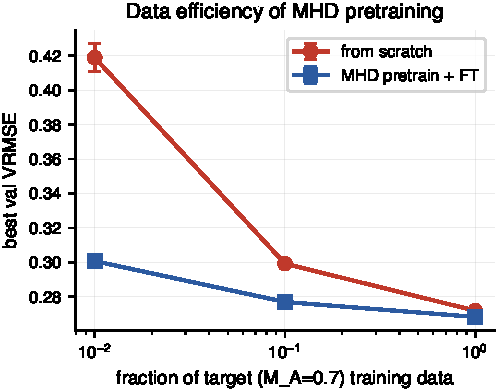
\includegraphics[width=0.55\linewidth]{figures/fig2_data_efficiency.pdf}
  \caption{Data efficiency of MHD pretraining. Error bars are standard deviation across 3 seeds for \{10\%, 1\%\} configurations (single-seed at 100\%). Baseline point at 1\% reflects the best-tuned configuration from a coarse hyperparameter sweep; raw untuned baseline (not shown) is 0.557.}
  \label{fig:data-eff}
\end{figure}

\subsection{The transfer is physics-specific: wrong physics hurts}

\begin{figure}[t]
  \centering
  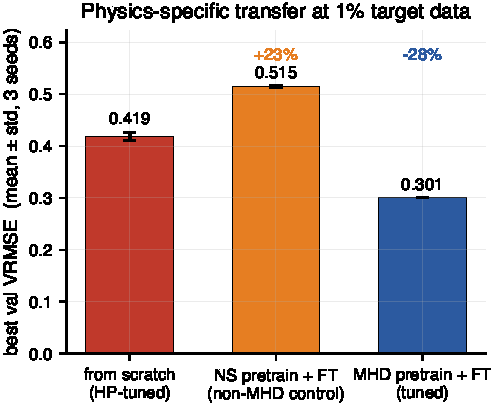
\includegraphics[width=0.62\linewidth]{figures/fig1_headline_physics_specificity.pdf}
  \caption{Physics-specific transfer at 1\% target data. Non-MHD pretraining on supernova radiation-hydrodynamics ($+23\%$ over scratch) is worse than training from scratch; only MHD pretraining produces a meaningful advantage ($-28\%$ over scratch). The 42\% difference between the two pretrain choices measures MHD-physics-specific transfer, cleanly separated from any architecture-level effect.}
  \label{fig:headline}
\end{figure}

The most natural alternative explanation for the 28\% advantage is that \emph{any} pretraining regularizes the network --- the source physics does not matter. To test this, we pretrained an identical-architecture FNO3D on Polymathic \texttt{supernova\_explosion\_64} (non-MHD 3D radiation-hydrodynamics) and fine-tuned on the same M$_A$=0.7 1\% target data. Figure~\ref{fig:headline} shows the result: wrong-physics pretraining \emph{hurts} target performance by 23\% compared to training from scratch. The 42\% gap between MHD and NS pretraining is the component of the transfer attributable to MHD-specific physics rather than to architecture-level regularization. The regularization-only hypothesis is falsified.

\subsection{What specifically transfers: spatial statistics, not temporal dynamics}

\paragraph{Perpendicular cascade (transfers).} Figure~\ref{fig:cascade} plots $E(k_\perp | k_\parallel \to 0)$ --- the perpendicular turbulent cascade for $B_x$ --- for one-step predictions on held-out M$_A$=0.7 trajectories. At 1\% target data, the from-scratch baseline loses high-$k_\perp$ power by nearly two orders of magnitude beyond $k_\perp \geq 8$. The MHD-pretrained fine-tuned model tracks ground truth across 1.5 decades of $k_\perp$. The Goldreich-Sridhar~\cite{goldreich1995theory} $k_\perp^{-5/3}$ reference slope is included for context.

\begin{figure}[t]
  \centering
  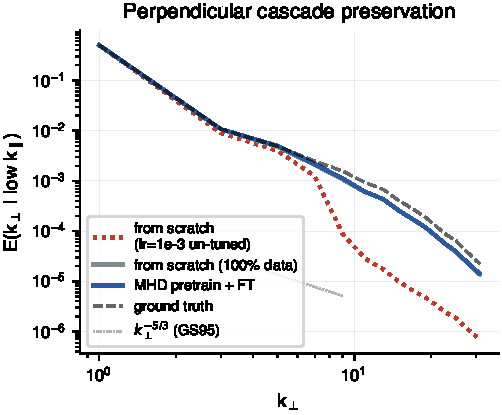
\includegraphics[width=0.55\linewidth]{figures/fig3_cascade.pdf}
  \caption{Perpendicular turbulent cascade. From-scratch at 1\% data fails to preserve high-$k_\perp$ structure; MHD pretrain + fine-tune matches ground truth and closely tracks the 100\%-data baseline.}
  \label{fig:cascade}
\end{figure}

\paragraph{Long-horizon rollout (fails, and differently).} Figure~\ref{fig:rollout} plots autoregressive rollout VRMSE versus step. The from-scratch 1\%-data model drifts smoothly to $\approx$2.0 and stabilizes there --- it has collapsed to a blurry, low-variance state that is stable because it barely evolves. The pretrained fine-tuned model is much better at short horizons (step 1 VRMSE 0.31 vs 0.56) but diverges explosively past step 20, reaching $\sim$16 by step 50 --- 8$\times$ worse than the undertrained scratch baseline. The two models fail in opposite directions: the scratch model collapses, the pretrained model inflates.

\begin{figure}[t]
  \centering
  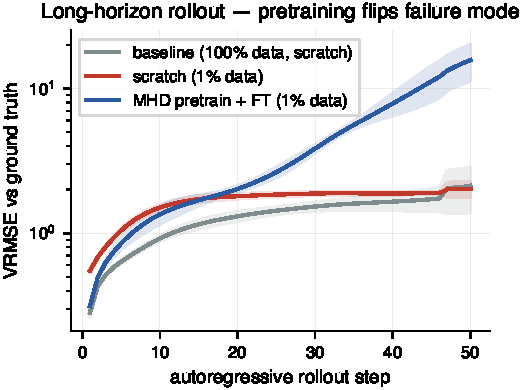
\includegraphics[width=0.55\linewidth]{figures/fig4_long_horizon_failure.pdf}
  \caption{Autoregressive rollout VRMSE vs step. Pretraining flips the long-horizon failure mode: rather than smoothing to a low-variance attractor (red), the pretrained fine-tuned model (blue) evolves dynamics confidently toward an increasingly wrong state, with whole-spectrum energy inflation.}
  \label{fig:rollout}
\end{figure}

\paragraph{Pretrain bias persists through fine-tuning.} In driven sub-Alfv\'enic MHD turbulence, the magnetic-to-kinetic energy partition follows $E_B/E_K \sim 1/M_A^2$: $\approx$2 for our M$_A$=0.7 target, $\approx$0.25 for the M$_A$=2.0 source. Figure~\ref{fig:equipartition} tracks this ratio during autoregressive rollout. The from-scratch baseline at 100\% data tracks the truth curve near 2.0 modulo noise; the from-scratch 1\%-data baseline undershoots slightly. \emph{The fine-tuned model drops rapidly from the M$_A$=0.7 target value, passes through the source-regime M$_A$=2.0 value, and overshoots.} This is direct evidence that fine-tuning on 1\% target data does not rewrite the statistical structure encoded during pretraining; the pretrain-regime equipartition persists and compounds during rollout.

\begin{figure}[t]
  \centering
  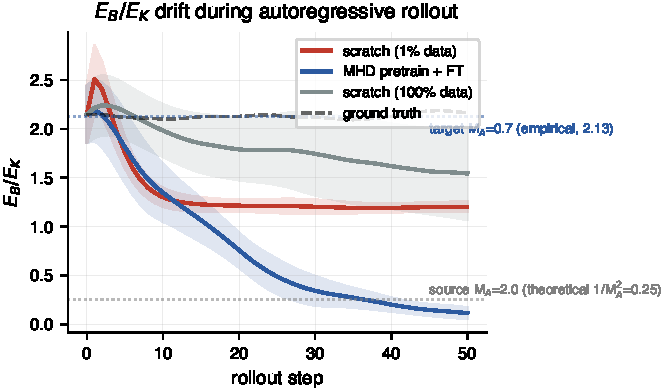
\includegraphics[width=0.55\linewidth]{figures/fig5_equipartition_drift.pdf}
  \caption{$E_B/E_K$ equipartition during autoregressive rollout. Horizontal dashed lines mark the theoretical ratios for the M$_A$=0.7 target regime ($\approx$2) and the M$_A$=2.0 pretrain regime ($\approx$0.25).}
  \label{fig:equipartition}
\end{figure}

\paragraph{Conservation violation.} Figure~\ref{fig:conservation} shows that the pretrained fine-tuned model violates $\nabla \cdot B = 0$ approximately 4$\times$ more than the from-scratch 1\%-data baseline, and that its magnetic energy drift accelerates past step 30 when the scratch baseline is stable. FNO3D is not architecturally conservation-preserving; pretraining exacerbates the existing architectural weakness rather than mitigating it.

\begin{figure}[t]
  \centering
  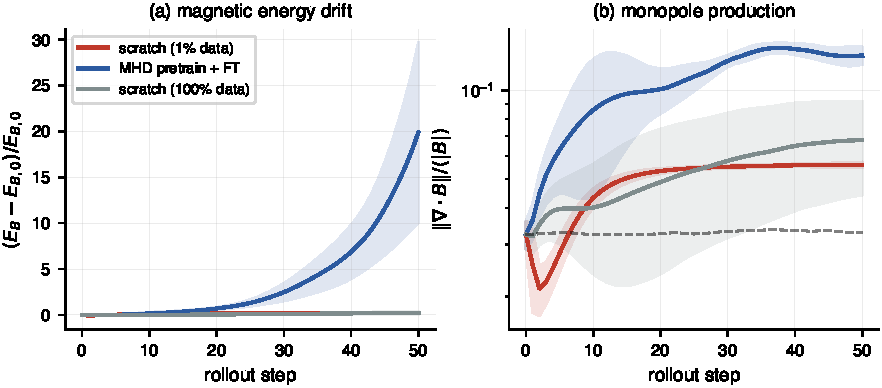
\includegraphics[width=0.95\linewidth]{figures/fig6_conservation_violation.pdf}
  \caption{Conservation violations during rollout. (a) Relative drift in magnetic energy $E_B$. (b) Magnetic monopole production $\|\nabla\cdot B\| / \langle |B| \rangle$ (log scale). The pretrained model produces more monopoles and accelerating energy drift compared to the undertrained scratch baseline, despite being more accurate at short horizons.}
  \label{fig:conservation}
\end{figure}

\section{Discussion}

Our three results, taken together, argue that \textbf{pretraining corpora for plasma foundation models must match target-domain physics, that the benefits of pretraining are concentrated in spatial-statistical structure rather than temporal dynamical stability, and that pretraining amplifies rather than mitigates architectural conservation weaknesses}. Three actionable implications follow.

\paragraph{Curating pretraining corpora for physics relevance.} The NS-pretrain control (Figure~\ref{fig:headline}) shows that pretraining on a physics regime that shares the governing architecture but not the governing equations actively harms downstream performance. A large, physics-agnostic scaling of pretraining compute will not automatically help; the corpus must include the physics of the target. For plasma applications, this strongly motivates plasma-specific pretraining datasets --- not just adding plasma as one of 20 domains in a broad corpus, but ensuring the plasma component is representative of the downstream regime family.

\paragraph{Architectural support for conservation and long-horizon stability.} The long-horizon rollout failure (Figures~\ref{fig:rollout} and~\ref{fig:conservation}) is architectural, not a data problem. Plasma emulators that need stable rollouts of tens of thousands of timesteps cannot rely on pretraining alone to impose the required inductive biases. Explicit constraints --- solenoidal projections for $B$, divergence-preserving update rules, conservation-aware loss terms, or hybrid pretraining that includes explicit long-rollout stability objectives --- are likely prerequisites. Our observation that \emph{pretraining makes} $\nabla\cdot B$ \emph{worse}, not better, rules out the optimistic reading that scale alone will eventually fix these issues.

\paragraph{The equipartition result as a diagnostic.} Figure~\ref{fig:equipartition}'s demonstration that fine-tuning does not rewrite the statistical structure of the pretraining regime suggests a practical diagnostic for assessing how much a fine-tuned plasma foundation model has actually adapted to its downstream task versus inherited the global statistical attractors of its pretraining data. For plasma applications where regime-specific quantitative accuracy matters (tokamak scenarios, astrophysical fits), this diagnostic is a useful sanity check independent of VRMSE scores.

\section{Limitations}

Our findings are conditional on a single architecture (FNO3D at 18.6\,M parameters) and a single dataset family (Polymathic \emph{Well} MHD\_64). The specific claim that transfer is physics-specific rests on one NS control dataset (supernova radiation-hydrodynamics); comparing to additional non-plasma controls would strengthen the result. The pretraining was run once per physics regime; multi-seed pretraining error bars would tighten the transfer estimates. The target regime is a simulation proxy (sub-Alfv\'enic MHD with an imposed $B_0$), not a tokamak or astrophysical-fit ground truth; cross-framework evaluation on data generated by different simulation codes (e.g., Athena++, Dedalus) is planned as follow-up work and is the natural setting for evaluating against transformer-based foundation models such as Walrus~\cite{mccabe2025walrus}, which we do not include here because the \texttt{MHD\_64} test split was part of Walrus's pretraining corpus and a clean out-of-distribution comparison requires data outside the Polymathic Well.

\section{Conclusion}

A narrow, physics-matched pretraining corpus produces a 28\% reduction in 1\%-data target VRMSE on sub-Alfv\'enic MHD, preserves the turbulent cascade, and is cheap. The same architecture pretrained on non-plasma physics is actively worse than scratch. But the pretrained model's long-horizon rollouts are catastrophically unstable relative to their short-horizon accuracy, and fine-tuning fails to rewrite pretraining's statistical biases. For plasma foundation models, these results argue for physics-aligned pretraining corpora and explicit architectural enforcement of conservation laws rather than relying on pretraining scale alone.

\small
\bibliographystyle{plain}
\bibliography{references}

\end{document}
